\section{Pre-Training}
 
\subsection{Architecture}

In the GLM-4.5 series, we adopt the MoE architecture, which improves the computational efficiency of both training and inference. We employ loss-free balance routing~\cite{wang2024auxiliary} and sigmoid gates for MoE layers~\cite{liu2024deepseek}. Different from DeepSeek-V3~\cite{liu2024deepseek} and Kimi K2~\cite{team2025kimi}, we reduce the width (hidden dimension and number of routed experts) of the model and increase its height (number of layers), as we found that deeper models exhibited better reasoning capacity. In the self-attention component, we employ Grouped-Query Attention with partial RoPE. Furthermore, we utilize 2.5 times more attention heads (96 heads for a 5120 hidden dimension). Counterintuitively, while this increased head count does not improve training loss compared to models with fewer heads, it consistently improves performance on reasoning benchmarks such as MMLU and BBH. We also incorporate QK-Norm~\cite{henry2020querykeynormalizationtransformers} to stabilize the range of attention logits. For both GLM-4.5 and GLM-4.5-Air, we add an MoE layer as the MTP (Multi-Token Prediction) layer~\cite{gloeckle2024mtp} to support speculative decoding during inference.

\begin{table}[!h]
    \centering
    \caption{Model architecture of GLM-4.5 and GLM-4.5-Air. When counting parameters, for GLM-4.5 and GLM-4.5-Air, we include the parameters of MTP layers but not word embeddings and the output layer.}
    
    \label{tab:placeholder}
    % \resizebox{\textwidth}{!}{
    \begin{tabular}{l|cc|cc}
    \toprule
       Model & \textbf{GLM-4.5} & \textbf{GLM-4.5-Air} & \textbf{DeepSeek-V3} & \textbf{Kimi K2} \\
    \midrule
       \# Total Parameters & 355B & 106B & 671B & 1043B \\
       \# Activated Parameters & 32B & 12B & 37B & 32B \\
       \# Dense Layers  & 3 & 1 & 3 & 1 \\
       \# MoE Layers & 89 & 45 & 58 & 60 \\
       \# MTP Layers & 1 & 1 & 1 & 0 \\
       Hidden Dim & 5120 & 4096 & 7168 & 7168 \\
       Dense Intermediate Dim & 12288 & 10944 & 18432 & 18432 \\
       MoE Intermediate Dim & 1536 & 1408 & 2048 & 2048 \\
       Attention Head Dim & 128 & 128 & 192 & 192\\
       \# Attention Heads & 96 & 96 & 128 & 64 \\
       \# Key-Value Heads & 8 & 8 & 128 & 64 \\
       \# Experts (total) & 160 & 128 & 256 & 384 \\
       \# Experts Active Per Token & 8 & 8 & 8 & 8\\
       \# Shared Experts & 1 & 1 & 1 & 1\\
       QK-Norm & Yes & No & No & No \\
       % Routed Expert Scaling Factor & 2.5 & 1\\
       % Vocabulary Size & 151552 & 151552\\
    \bottomrule
    \end{tabular}
    % }
\end{table}


\subsection{Pre-Training Data}
Our pre-training corpus includes documents from webpages, social media, books, papers, and code repositories. We carefully design the data processing pipelines for different sources. 

\paragraph{Web} The majority of our pre-training documents are English and Chinese webpages crawled from the Internet. Inspired by Nemotron-CC~\cite{su2024nemotron}, we divide the crawled webpages into buckets of different quality scores. We up-sample documents from the bucket with higher quality scores
and discard documents from the bucket with the lowest quality scores. The bucket with the highest quality scores contributes over 3.2 epochs during pre-training. In this way, the pre-training corpus can emphasize the high-frequency knowledge for reasoning tasks and also improve coverage for long-tail world knowledge. We have also found a large number of similar webpages automatically generated from templates and assigned high scores. Such webpages cannot be removed by MinHash deduplication. We additionally apply the SemDedup~\cite{abbas2023semdedup} pipeline to remove those similar webpages based on document embeddings.

\paragraph{Multilingual} To support more natural languages, we include multilingual documents in our pre-training corpus. The multilingual corpus comes from both our crawled webpages and Fineweb-2~\cite{penedo2025fineweb2}. We apply a quality classifier that judges the educational utility of documents and up-sample high-quality multilingual documents.

\paragraph{Code} We curated source code data from GitHub and various code hosting platforms. The code corpus undergoes a preliminary rule-based filtering, followed by classification using language-specific quality models that categorize samples into three tiers: high-quality, medium-quality, and low-quality. During training, we up-sampled high-quality code while excluding low-quality samples. Moreover, the Fill-In-the-Middle~\cite{bavarian2022efficienttraininglanguagemodels} training objective is applied to all source code data. 
For code-related web documents, we employ a two-stage retrieval process from our text pre-training corpus. Documents are initially selected based on two criteria: presence of HTML code tags, or identification by a FastText~\citep{joulin2017bag} classifier trained to detect code-related content. Subsequently, the retrieved documents undergo quality assessment using a dedicated model that classifies them into high-, medium-, or low-quality categories, following the same quality-based sampling strategy for source code. Finally, a fine-grained parser is employed to re-parse the selected web pages to better preserve the formats and contents of the code.

\paragraph{Math \& Science} To enhance the reasoning capacity, we collect documents related to mathematics and science from webpages, books, and papers. We apply a large language model to score candidate documents based on the ratio of educational content about mathematics and science, and train a small-scale classifier to predict the scores. Documents in the pre-training corpus with scores above a certain threshold are up-sampled.

The pre-training process of GLM-4.5 is divided into two stages. In the first stage, the model is mainly trained on general documents from webpages. During the second stage, we up-sample the source code from GitHub and webpages related to coding, mathematics, and science.

\subsection{Mid-Training: Boost Reasoning \& Agentic Capacity}

\begin{figure}
    \centering
    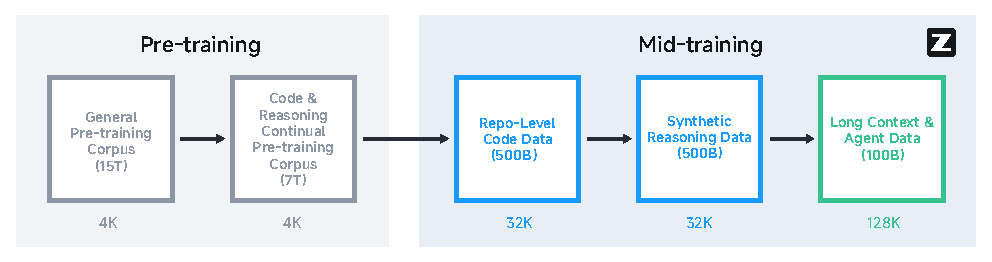
\includegraphics[width=\linewidth]{figures/pretrain.pdf}
    \caption{Pre-training and mid-training stages for GLM-4.5. We adapt a multi-stage training recipe and extend the sequence length from 4K to 128K.}
    \label{fig:pretrain}
\end{figure}

After pre-training, we add several stages to further boost the model's performance on important application areas. Unlike traditional pre-training on large-scale general documents, these training stages utilize medium-size domain-specific datasets, including instruction data. Therefore, we denote these training stages as mid-training, which includes the following.

\paragraph{Repo-level Code Training} At this training stage, we add concatenated code files from the same repository to learn cross-file dependency. To improve the model's software engineering capability, we also include model-filtered issues, pull requests (PRs), and commits from GitHub, with related issues, PRs, and commits concatenated into one context and commits organized in a diff-like format. We extend the training sequence length from 4K to 32K to incorporate large repositories.

\paragraph{Synthetic Reasoning Data Training} At this stage, we add synthetic reasoning content for math, science, and coding competitions. We collect a large number of questions and answers related to the reasoning tasks from webpages and books, and synthesize reasoning processes with a reasoning model.
\paragraph{Long-context \& Agent Training} To further boost the model's long-context performance, we extend the training sequence length from 32K to 128K and up-sample long documents from the pre-training corpus. Large-scale synthetic agent trajectories are also incorporated at this stage.

In \Cref{fig:pretrain}, we show the complete stages for pre-training and mid-training. The maximum sequence length is kept at 4,096 in pre-training, and is extended from 32,768 to 131,072 in mid-training. During pre-training, we did not use best-fit packing~\cite{ding2024fewer} since random truncation is a good data-augmentation strategy for pre-training documents. For datasets in mid-training, we applied best-fit packing to avoid truncating the reasoning process or repo-level code.

\subsection{Hyper-Parameters}

We employed the Muon optimizer~\cite{jordan6muon,liu2025muon} for all parameters except word embedding, bias, and weights for RMSNorm. For hyperparameters, we set the Newton-Schulz iteration steps $N$ to 5, momentum $\mu$ to 0.95, and scaled Muon's update RMS to 0.2. We observed that the Muon optimizer can accelerate convergence and tolerate larger batch sizes. We used cosine decay schedule for learning rate, instead of warmup-stable-decay (WSD) schedule~\cite{huminicpm}. Our early experiments showed that models trained with the WSD schedule perform worse on general benchmarks (SimpleQA, MMLU), indicating underfitting in the stable stage. The learning rate went through a warm-up stage from 0 to 2.5e-4 and a decaying stage to 2.5e-5 until the end of mid-training. We used a batch size warmup strategy, where the batch size was gradually increased from 16M tokens to 64M tokens in the training of the first 500B tokens, and remained constant in the remaining of training. 
For regularization, we set the weight decay ratio to 0.1 and did not use dropout. We set the maximum sequence length to 4,096 during pre-training, and extended it to 32,768 and 131,072 during the mid-training stage as shown in~\Cref{fig:pretrain}. When extending the sequence length to 32K, we also adjusted RoPE's base frequency from 10,000 to 1,000,000 for better long-context modeling ability. For loss-free balance routing, we set the bias update rate to 0.001 for the first 15T tokens, and to 0.0 for the remaining tokens. We also applied auxiliary sequence-level balance loss with a 0.0001 weight to avoid extreme imbalance within any single sequence. The MTP loss weight $\lambda$ was set to 0.3 for the first 15T tokens, and to 0.1 for the remaining tokens.
